\section{Performance}

\begin{quote}
    {\em A well designed Lustre storage system can achieve
    90\% of underlining hardware bandwidth.}
    \flushright{\scriptsize--- Zhiqi Tao, Sr. System Engineer, Intel \cite{10-intel}}
\end{quote}

\tikzset {
    graph/.style = {
        mark=x,
        line width=1pt,
        line cap=round,
    },
}

\subsection{Theoretical Limits}

    In the following table, I present a theoretical Lustre environment setup
    with some key specifications, and the resulting, theoretical limits. These
    calculated values of course do not contain any performance limitations such
    as overhead, metadata access, or network capabilities, but rather show
    what would be the absolute limit.

    \begin{tabular}{|l|l|}
        \hline
        System specifications & Theoretical performance \\\hline
        \renewcommand{\arraystretch}{1.1}
        \begin{tabular}[t]{ll}
            \textbf{OSS count}       & 160 \\
            \textbf{OST/OSS}         & 16  \\
            \textbf{OST size}        & 2 TiB  \\
            \textbf{OST throughput}  & 50 MiB/s
        \end{tabular} &
        \renewcommand{\arraystretch}{1.1}
        \begin{tabular}[t]{ll}
            \textbf{Total storage}      & 2.5 PiB (Pebibyte) \\
            \textbf{Throughput per OSS} & 800 MiB/s  \\
            \textbf{Total throughput}   & 125 GiB/s
        \end{tabular}
        \renewcommand{\arraystretch}{1.5}
        \\\hline
    \end{tabular}

    Due to the Lustre architecture, the resulting values come close to the
    presented limits. There are only a few bottlenecks that still remain, and
    these are actively being improved.

\subsection{Recent Improvements}

\subsubsection{ZFS support}

ZFS support comes with many improvements. Mainly, it allows for new kernels to
run the servers without patching required. Furthermore, ZFS is more widely used
by the open source community, thus being more actively developed and supported
by a wider user base.

More ZFS features include checksums, support for up to 256 ZiB (Zebibyte,
$10^21$ Bytes) storage per OST, compression support and copy-on-write. All of
these assist the performance and possibilities of a Lustre system.

\subsubsection{Wide Striping}

Until recently, the number of OSTs that stored a single file was limited to 160,
due to the number of records available in an inode. This limit has been breached
by storing the information in the extended attributes (``xattrs'') array of the
inode. ZFS also does not have this limit.

\subsubsection{Multiple MDS}

Since metadata access used to be the main performance bottleneck, work has been
focused on improving this. Since Lustre 2.4, more than one simultaneous MDS
are supported. This is implemented by either striping the metadata across
multiple targets, similar to object striping, or namespacing the metadata. In a
namespaced environment, some subtree (directory) of the file system would be
handled by a different MDS, thus splitting the load.

These two methods provide a good way of fine-tuning the metadata system by the
administrator according to the needs of the clients.

\subsubsection{Metadata overhead}

A common task in file system operation is directory traversal (\texttt{readdir})
and metadata readout (\texttt{stat}). This combination is used, for example, in
the UNIX command \texttt{ls -l}.

The problem with this approach is that for each file in the directory, a separate
RPC (\texttt{stat}) has to be sent and processed. This creates a lot of network
overhead and I/O wait for directories with many files.

One solutions is the non-standard \texttt{readdirplus} command from the POSIX
HPC I/O Extensions \cite{posix-ext}. Lustre implements this extensions, and sents
a single response including the metadata of the files.

Since not every client supports the HPC I/O Extensions, the Lustre MDS also
detects a combination of \texttt{readdir} and \texttt{stat} calls and requests
all stats from OSSs in advance, parallelized, then sending a combined RPC reply
that can be up to 1 MiB in size.

The following graphs visualize the metadata performance of both the original
POSIX directory traversal, and the improved Lustre detection system. One can
see that the improved version is up to 27x faster (y-axis in log scale) than
the original one on files that are striped across 4 OSSs, since the metadata is
fetched in parallel.

\vspace{0.5cm}

\makebox[0.5\textwidth][c] {
    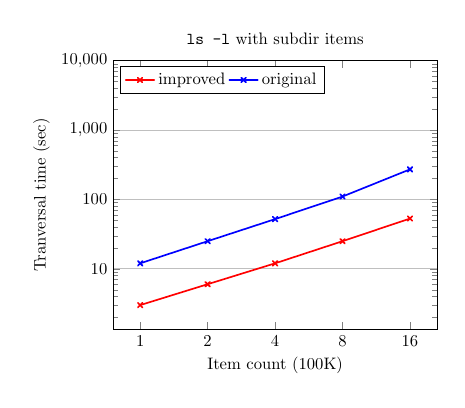
\begin{tikzpicture}[scale=0.6]
        \begin{loglogaxis}[
            xlabel={Item count (100K)},
            log basis x=2,
            xticklabel=\pgfmathparse{2^\tick}\pgfmathprintnumber{\pgfmathresult},
            ylabel={Tranversal time (sec)},
            yticklabel=\pgfmathparse{10^\tick}\pgfmathprintnumber{\pgfmathresult},
            log basis y=10,
            legend style={at={(0.02,0.98)},anchor=north west,cells={anchor=west}},
            legend columns=3,
            title={\texttt{ls -l} with subdir items},
            ymajorgrids,
            ymin=0,ymax=10000,
            ]
            %\axispath\draw
                    %(7.49165,-10.02171)
                %|-  (8.31801,-11.32467)
                %node[near start,left] {$\frac{dy}{dx} = -1.58$};

            \addplot[graph,color=red] plot coordinates {
                (1, 3)
                (2, 6)
                (4, 12)
                (8, 25)
                (16, 53)
            };
            %
            \addlegendentry{improved}

            \addplot[graph,color=blue] plot coordinates {
                (1, 12)
                (2, 25)
                (4, 52)
                (8, 110)
                (16, 271)
            };
            \addlegendentry{original}
        \end{loglogaxis}
    \end{tikzpicture}
}\makebox[0.5\textwidth][c] {
    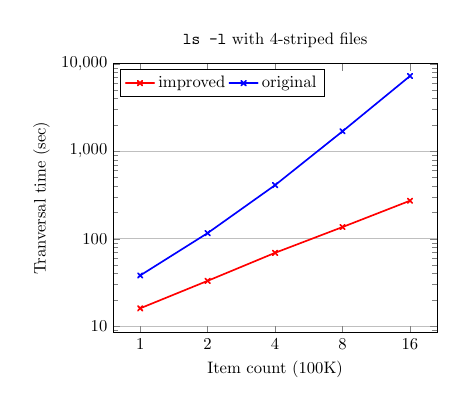
\begin{tikzpicture}[scale=0.6]
        \begin{loglogaxis}[
            xlabel={Item count (100K)},
            log basis x=2,
            xticklabel=\pgfmathparse{2^\tick}\pgfmathprintnumber{\pgfmathresult},
            ylabel={Tranversal time (sec)},
            yticklabel=\pgfmathparse{10^\tick}\pgfmathprintnumber{\pgfmathresult},
            log basis y=10,
            legend style={at={(0.02,0.98)},anchor=north west,cells={anchor=west}},
            legend columns=3,
            title={\texttt{ls -l} with 4-striped files},
            ymajorgrids,
            ymin=0,ymax=10000,
            ]
            %\axispath\draw
                    %(7.49165,-10.02171)
                %|-  (8.31801,-11.32467)
                %node[near start,left] {$\frac{dy}{dx} = -1.58$};

            \addplot[graph,color=red] plot coordinates {
                (1, 16)
                (2, 33)
                (4, 69)
                (8, 136)
                (16, 272)
            };
            \addlegendentry{improved}

            \addplot[graph,color=blue] plot coordinates {
                (1, 38)
                (2, 116)
                (4, 410)
                (8, 1692)
                (16, 7248)
            };
            \addlegendentry{original}
        \end{loglogaxis}
    \end{tikzpicture}
}

\hfill{\scriptsize\emph{graph data from \cite{metadata-scaling}}}

\subsubsection{SSDs as MDT}

Since metadata performance is still the major bottleneck, suggestions have been
made to better support solid state drives (SSDs) as metadata targets. These have
a higher throughput, but most importantly an order of magnitude more IOPS, which
is important for metadata seeks. Furthermore, the metadata storage requires
relatively low capacity, which makes using the more expensive SSDs for MDTs
affordable.

The graphs in Figure~\ref{fig:ssds} visualize the analysis of different drive types for metadata
storage for the three main metadata operations (create, stat, unlink). They were
measured using both ldiskfs and ZFS (in development) versions, using 8
processes per client node.

The data shows that generally, the ZFS branch achieved the lowest performances.
Since this is an early development branch (Orion-Lustre), recent improvements
have to be expected. Furthermore, the ldiskfs-RAM line (green) displays the
limit of what can be achieved independent of the drive used. One can notice that
SSDs are better than HDDs, but not by the expected order of magnitude. Some
research can be expected in this area. Also quite noticable is the apparent limit
of stat calls per second, not rising above \textasciitilde50,000, not even in RAM.
This seems to be another bottleneck, where metadata striping or namespacing may
yield better results due to distribution of the load across multiple servers.

\newcommand{\ssd}[2]{
    \scriptsize
    \center
    \begin{tikzpicture}
        \begin{semilogxaxis}[
            xlabel={Client nodes},
            log basis x=2,
            ylabel={#1 per second},
            legend style={font=\tiny,at={(0.02,0.98)},anchor=north west,cells={anchor=west}},
            legend columns=2,
            scaled ticks=false,
            ymajorgrids,
            %xticklabel=\pgfmathparse{2^\tick}\pgfmathprintnumber{\pgfmathresult},
            xtick={0.5,1,2,4,8,16},
            xticklabels={Single Node,1,2,4,8,16},
            width=\textwidth,
            height=7.5cm,
            ]
            %\axispath\draw
                    %(7.49165,-10.02171)
                %|-  (8.31801,-11.32467)
                %node[near start,left] {$\frac{dy}{dx} = -1.58$};
            \addplot[graph,unbounded coords=jump,color=red]    table [y index=1] {data/#2.csv}; \addlegendentry{ldiskfs-HDD}
            \addplot[graph,unbounded coords=jump,color=Dandelion] table [y index=2] {data/#2.csv}; \addlegendentry{ldiskfs-SSD}
            \addplot[graph,unbounded coords=jump,color=green]  table [y index=3] {data/#2.csv}; \addlegendentry{ldiskfs-RAM}
            %\addplot[graph,unbounded coords=jump,color=purple] table [y index=5] {data/#2.csv}; \addlegendentry{ldiskfs-SSD-SD}
            \addplot[graph,unbounded coords=jump,color=blue]   table [y index=6] {data/#2.csv}; \addlegendentry{ZFS-SSD}
        \end{semilogxaxis}
    \end{tikzpicture}
}

\begin{figure}
    \ssd{Creates}{ssd-create}
    \ssd{Stats}{ssd-stat}
    \ssd{Unlinks}{ssd-unlink}
    \centering
    \caption{Metadata performance by number of clients using different drive types \cite{mds-eval}}
    \label{fig:ssds}
\end{figure}
